\documentclass[11pt,a4paper]{article}
\usepackage{tikz}
\usetikzlibrary{arrows.meta,positioning}
\usepackage{tabularx}
\usepackage{amsmath,amssymb,amsthm}
\usepackage{geometry}
\geometry{margin=1in}
\usepackage{hyperref}
\usepackage{graphicx}
\usepackage{setspace}
\onehalfspacing

\title{\textbf{Paper B-03: Information Flow and Digital Infrastructure:\\ A Constraint-Driven Flux Dynamics (CDFD) Perspective}}
\author{Steve Bico Mujjabi, MD\\
\small Independent Researcher\\
\small Founder, Vura Labs\\
\small Kampala, Uganda\\
\small ORCID: 0009-0001-0556-5516}
\date{August 2026}

\begin{document}
\maketitle

% BEGIN SHARED-METHODS POINTER
\noindent\textit{Shared Part IV notation and evidence boundaries are defined in \path{PART_IV_METHODS_AND_CLAIM_BOUNDARY.md}. This paper states only its local observables, comparison, and failure conditions.}
% END SHARED-METHODS POINTER


\begin{abstract}
This paper develops a falsifiable CDFD/AFL model of Internet Routing. It maps packet demand, route announcements, and application traffic to driving flux $\Phi$, bandwidth, queue capacity, latency, policy, and physical links to active constraint $C$, routing, congestion control, caching, and traffic engineering to responsiveness $S$, and cached state, route history, failure scars, and protocol configuration to structural memory $M_s$. The target outcome is throughput, delay, loss, reachability, and recovery, tested against packet traces, queue telemetry, routing tables, topology, and outage records. The paper treats universality as a shared model architecture rather than an assertion that unlike systems have the same material mechanism. It states the negative result that would make the mapping unnecessary and places the domain claim inside the cumulative CDFD programme and its reproducible runtime boundary.
\end{abstract}
% BEGIN CONSOLIDATION SCOPE
\section*{Consolidation Scope and Provenance}
This consolidated paper incorporates internet routing, computational architecture, and digital information-flow scopes formerly carried by Papers B-03, B-11, and D-10. Routing performance, system utilization, and information diffusion are distinct outcomes and must not be collapsed into one threshold.
% END CONSOLIDATION SCOPE


\section{Introduction}

The internet is an unprecedented experiment in macroscopic information transport. When a user requests a video stream, the data is sliced into packets and fired across optical fibers, dynamically navigating around severed cables and overloaded servers to reach its destination.

Unlike the electrical grid, which has a rigid physical topology, the internet possesses high software plasticity. However, the physical hardware underlying the web still enforces hard thermodynamic and capacity constraints. The internet is a living CDFD surface, constantly breathing in data flux and exhaling information.

\section{The Network as an Adaptive Surface}
We evaluate the health of a data center or routing node via the Adaptive Operating Ratio:
\begin{equation}
    \Psi_s = \left( \frac{\Phi}{C} \right) \cdot S \cdot M_s
\end{equation}

For an autonomous internet node:
\begin{itemize}
    \item \textbf{Flux ($\Phi$)}: The gigabits per second of incoming and outgoing data packets.
    \item \textbf{Constraint ($C$)}: The physical bandwidth limits of the fiber optic cables and the processing friction (latency) of the routers.
    \item \textbf{Responsiveness ($S$)}: The node's buffer memory capacity and the elasticity of its load-balancing algorithms, allowing it to temporarily absorb traffic spikes.
    \item \textbf{Memory ($M_s$)}: The Border Gateway Protocol (BGP) routing tables and DNS caches. If routing tables are updated too slowly, the network "remembers" obsolete paths, locking the system's topology into an inefficient state.
\end{itemize}

\subsection{congestion (chronic $C$ saturation) Collapse and BGP Failures}
A healthy router operates at $\Psi_s \approx 1$, passing packets ($\Phi$) as fast as they arrive without violating its bandwidth constraints ($C$).

Consider a Distributed Denial of Service (DDoS) attack. A massive, artificial spike in flux $\Phi$ hits the target node. The physical constraint $C$ remains fixed. The node's responsiveness $S$ (its packet buffer) fills up instantly. The adaptive ratio skyrockets ($\Psi_s \gg 1$). To protect the hardware and the network, the router simply drops the excess packets, functionally forcing the excess flux into dissipation.

A more insidious failure occurs via BGP misconfigurations. If an upstream ISP broadcasts a faulty route, the memory $M_s$ of millions of routers locks onto a "black hole" path. The local constraint $C$ effectively becomes infinite for that specific traffic flow. The adaptive ratio crashes ($\Psi_s \ll 1$). Data ceases to flow globally, not because of a physical hardware failure, but because the systemic memory has pathologically overridden the network's capacity to adapt.



\section{Measurement Layer}

% BEGIN PART IV MAJOR CROSS-DOMAIN UPGRADE
\section{Cross-Domain Model Upgrade: Mechanism, Scale, and Tests}

\subsection{Observable Translation}

The paper-specific translation begins with an observable chain rather than a
verbal analogy. For Internet Routing, the proposed drive is packet demand, route announcements, and application traffic.
The active limitation is bandwidth, queue capacity, latency, policy, and physical links. Responsiveness is carried by
routing, congestion control, caching, and traffic engineering, while retained state is represented by
cached state, route history, failure scars, and protocol configuration. The outcome to explain is throughput, delay, loss, reachability, and recovery.

\begin{table}[htbp]
\centering
\small
\caption{Operational CDFD/AFL map for Paper B-03.}
\begin{tabularx}{\textwidth}{|l|X|X|}
\hline
\textbf{Term} & \textbf{Paper-specific observable meaning} & \textbf{Measurement question} \\
\hline
$\Phi$ & packet demand, route announcements, and application traffic & What rate, load, gradient, or demand enters the focal system? \\
\hline
$C$ & bandwidth, queue capacity, latency, policy, and physical links & Which measured bottleneck limits transfer, function, or recovery? \\
\hline
$S$ & routing, congestion control, caching, and traffic engineering & Which process changes effective capacity or reroutes the load? \\
\hline
$M_s$ & cached state, route history, failure scars, and protocol configuration & Which retained state makes equal present loads produce different futures? \\
\hline
$Y$ & throughput, delay, loss, reachability, and recovery & Which outcome is predicted out of sample, with uncertainty? \\
\hline
\end{tabularx}
\end{table}

\begin{figure}[htbp]
\centering
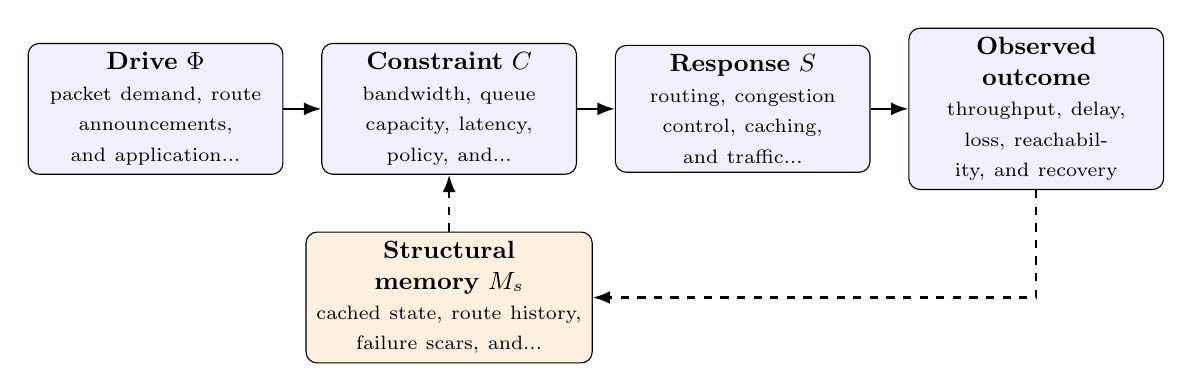
\begin{tikzpicture}[
    node distance=0.48cm,
    every node/.style={font=\small},
    box/.style={draw, rounded corners, align=center, minimum height=1.45cm, text width=3.0cm, fill=blue!6},
    memory/.style={draw, rounded corners, align=center, minimum height=1.25cm, text width=3.4cm, fill=orange!12},
    flow/.style={-{Latex[length=2.2mm]}, thick},
    feedback/.style={-{Latex[length=2.2mm]}, thick, dashed}
]
\node[box] (drive) {\textbf{Drive $\Phi$}\\\scriptsize packet demand, route announcements, and application...};
\node[box, right=of drive] (constraint) {\textbf{Constraint $C$}\\\scriptsize bandwidth, queue capacity, latency, policy, and...};
\node[box, right=of constraint] (response) {\textbf{Response $S$}\\\scriptsize routing, congestion control, caching, and traffic...};
\node[box, right=of response] (outcome) {\textbf{Observed outcome}\\\scriptsize throughput, delay, loss, reachability, and recovery};
\node[memory, below=0.72cm of constraint] (memory) {\textbf{Structural memory $M_s$}\\\scriptsize cached state, route history, failure scars, and...};
\draw[flow] (drive) -- (constraint);
\draw[flow] (constraint) -- (response);
\draw[flow] (response) -- (outcome);
\draw[feedback] (outcome.south) |- (memory.east);
\draw[feedback] (memory.north) -- (constraint.south);
\end{tikzpicture}
\caption{Paper B-03 observable CDFD/AFL architecture for Internet Routing. Solid arrows give the proposed forward chain; dashed arrows make history-dependent feedback explicit.}
\label{fig:b03-architecture}
\end{figure}

\subsection{Paper-Specific Causal Hypothesis}

For this paper, the hypothesized causal sequence is specific. A change in
packet demand, route announcements, and application traffic arrives faster than routing, congestion control, caching, and traffic engineering can compensate.
This raises or redistributes bandwidth, queue capacity, latency, policy, and physical links. If the load persists,
the retained state encoded by cached state, route history, failure scars, and protocol configuration changes the next response, so a later event of equal
magnitude can produce a different trajectory in throughput, delay, loss, reachability, and recovery. The
scientific task is to estimate that sequence against the best ordinary model of
the domain, not merely to redescribe the outcome after it occurs.

\subsection{Cross-Scale Translation Without Mechanistic Erasure}

For the engineered systems family, the cross-domain translation compares demand, designed capacity, feedback control, dependency topology, and accumulated technical state. The strongest engineering use is prospective: the mapping must identify a bottleneck, a control action, or a recovery signature before the failure occurs. \cite{BarabasiAlbert1999,WattsStrogatz1998,Shannon1948,BakTangWiesenfeld1987}
The required scale declaration for this paper is microseconds to years; flows to the global Internet. At short
scales, the key question is whether the incoming drive is transmitted,
buffered, or diverted. At intermediate scales, response changes effective
capacity and network exposure. At long scales, retained structure can alter the
state space itself. A result is genuinely cross-scale only when the aggregation
rule is stated and the same conclusion is not an artifact of averaging.

\subsection{Evidence Ladder and Discriminating Tests}

\begin{table}[htbp]
\centering
\small
\caption{Evidence ladder for Paper B-03. Each rung can fail independently.}
\begin{tabularx}{\textwidth}{|p{0.17\textwidth}|X|X|}
\hline
\textbf{Test} & \textbf{Design} & \textbf{Discriminating result} \\
\hline
Proxy audit & Measure packet traces, queue telemetry, routing tables, topology, and outage records and preregister how each record maps to $\Phi$, $C$, $S$, $M_s$, and $Y$. & The mapping fails if proxies are non-identifiable, circular, or change meaning across cases. \\
\hline
Load ramp & Apply or observe a traffic surge combined with a route or link failure while estimating the dominant constraint and response time. & A threshold claim requires a reproducible nonlinear change and uncertainty bounds, not a visually chosen breakpoint. \\
\hline
Recovery and memory & Match present load across units with different histories, then compare recovery paths. & The memory claim requires history-dependent divergence after current conditions are controlled. \\
\hline
Model comparison & Compare the baseline domain model with and without the CDFD/AFL state variables using held-out data. & The paper's stated falsifier is: memory-aware terms do not improve congestion or recovery forecasts. \\
\hline
\end{tabularx}
\end{table}

\subsection{Research Programme and Boundary Conditions}

The immediate research programme has four steps. First, construct a documented
dataset from packet traces, queue telemetry, routing tables, topology, and outage records and retain raw units before normalization.
Second, fit a baseline domain model and report its calibration and out-of-sample
error. Third, add the smallest identifiable CDFD/AFL state extension and test
whether it improves prediction of throughput, delay, loss, reachability, and recovery. Fourth, repeat the
analysis across the declared scale range and publish negative cases as part of
the cross-domain translation audit.

% END PART IV MAJOR CROSS-DOMAIN UPGRADE

\section{Conclusion}
The internet is governed by a comparable flow-control logic as biological circulatory systems. TCP window scaling is essentially an algorithmic implementation of Adaptive Flux Limitation, natively seeking to keep $\Psi_s \approx 1$. By recognizing information transport as a CDFD phenomenon, we can design future decentralized networks that treat routing memory not as a static table, but as a fluid, thermodynamically responsive tissue.
\section*{Conflict of Interest} The author declares no conflict of interest.
\section*{Data Availability}
Part-specific runtime diagnostics are under each Part's \path{outputs/} directory.

Release-wide code: \path{Part_E_Synthesis/supplementary/}.

Generated summaries: \path{Part_E_Synthesis/outputs/}.

Figures: \path{Part_E_Synthesis/figures/}.


\section{Reference Layer}
\bibliographystyle{plain}
\bibliography{universal_afl_references}
\end{document}
